\section{Modelling the Earth}
In the previous section the air quality and its detrimental effects on human health was seen to influence polcicy for cities and industry. Koyoto, Islands suing powerstations.

For a policy to be passed there needs to not only evidence of the problem, but a strong suggestion that any proposed changes will have the desired effect. As it is not possible to perform experiments on complex, and often unknown, chemistry at every location on the planet, we are forced to rely on the numerical simulation of the Earth System, and the constituent parts within it.

\subsection{Earth System Models (ESM)}

  ESMs are models capable of predict past or future interactions of the planetary system. They represnt our foremost understanding of the complex interplay between land-surface (geosphere), ocean (hydrosphere), ice (cryosphere) and the air (atmosphere), and act as a surrogate to manual experimentation -  which is just not possible on the global scale.

ESMs can be split into their individial parts. One example of this is the Chemistry section of the Goddard Earth Observing System (an integrated ESM and data assimulation model hosted by NASAs Goddard space flight centre \citep{geoschem}) - GEOS Chem. GEOS-Chem is a global 3D model of atmospheric chemistry which is driven by the meteorology provided by NASA \citep{geos}. Here the earth is split up into cubic sphere cells longitudally and latitudally, as well as vertically (\autoref{fig:gcm})\footnote{This image is not from GEOS-Chem.}. Each one of these cells performs several purtubations of the chemistry within them, before any long-lived species are transported, and the process is repeated. If extracted separately a single one of these cells may be used to explore the sensetivity of different species for a range of input conditions. This is the bases of the atmospheric box model.

\begin{figure}
  \centering
  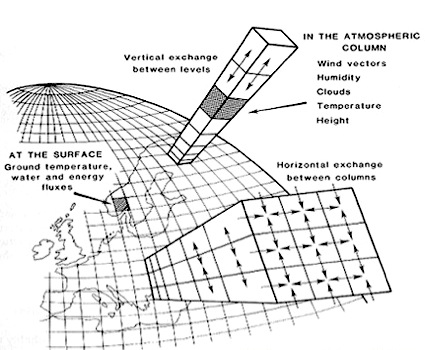
\includegraphics[width=0.6\textwidth]{gcm.jpg}
  \caption{\textbf{A diagram showing the longitudal, lateral and vertical decomposition of a 3D global model.} Source: \citep{gcm}}
  \label{fig:gcm}
\end{figure}


\subsection{The box model.}
In exploring the sensetivities of individual species within a simulation, it is possible to use a zero dimensional box model. This is in essence a single cell within the global structure, constrained in location and height (pressure).



mechanism,

integrator,

etc.






\subsubsection{Chemical Mechanisms}
Mechanisms are at the heart of every chemistry simulation. They are a mathematical representation of the possible reactions ( and the rates at which these may occur ) for every s


\begin{figure}
  \centering
  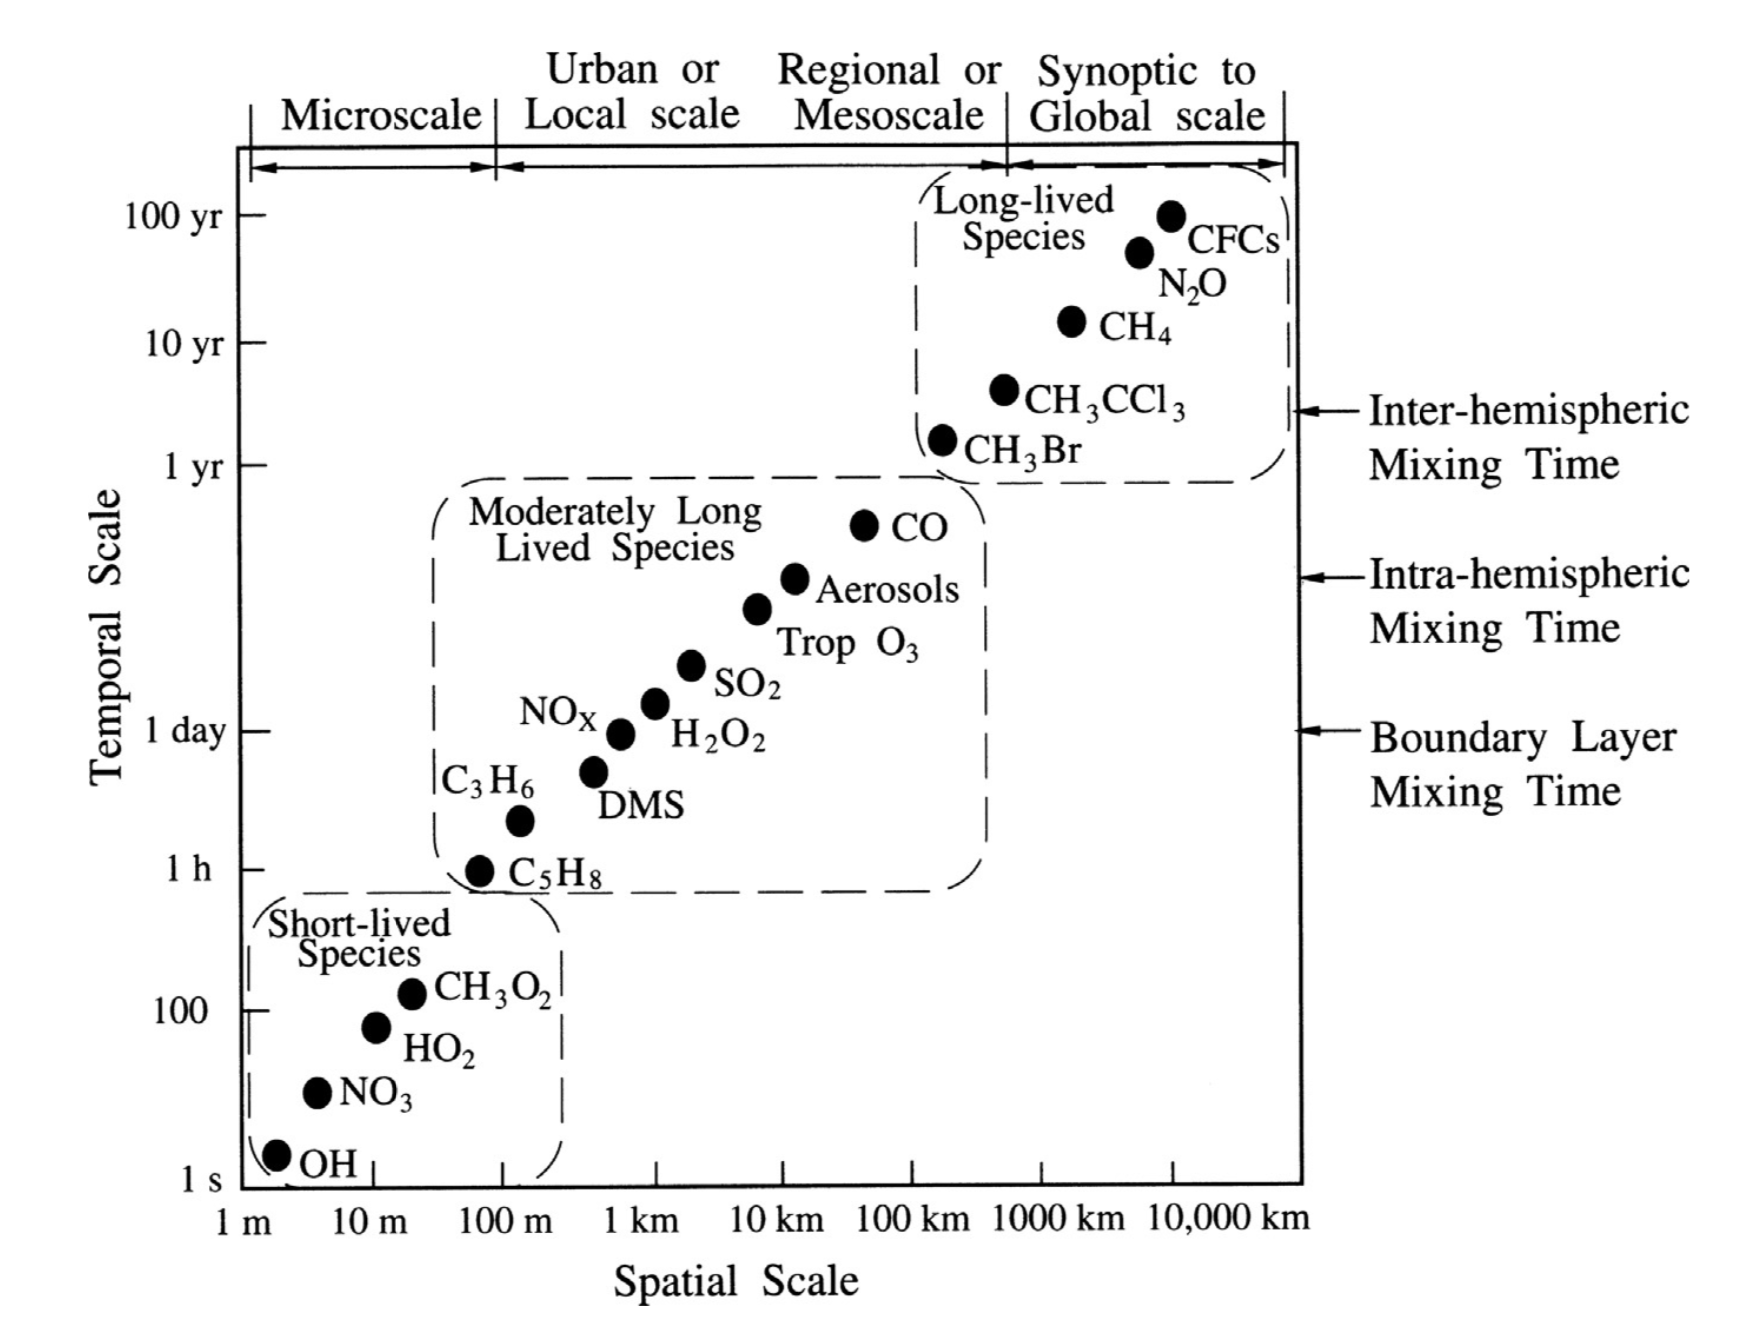
\includegraphics[width=0.7\textwidth]{timescales.png}
  \caption{\textbf{Spatial and temporal scales of variability of atmospheric species.} Source: \citep{transporttime}}
  \label{fig:timescales}
\end{figure}



The atmosphere consists of thousands of species, with tens of thousands of reactions between them.

These models represent real wodlc reactions


In modelling these we can describe their rate of production and loss with respect to the species they react with.



\subsection{Numerical integration}

For example, it is possible to figure out how quickly each species in a reaction is changing if the reaction mechanism (the exact way it happe ns) and some simple data are known. This representation of how quickly the concentrations are changing is the same as a slope, or derivative. Integration allows us to find the actual change over time and not just how quickly the change is happening. Fo r example, given the following reaction,

In a mechanism we are concerned with calculating how quickly a species changes within the chemical system. Taking the reaction of \ch{N2O5} (\autoref{eqn:numerical1}) we can write the rate of change for each species over time (\autoref{eqn:numerical2})\footnote{This is also known as the flux.}. In integrating this equation, we are able to calculate the actual change in concentration (\autoref{eqn:numerical3}) - this is the foundation of atmospheric models.

\begin{equation}
\ce{N2O5 ->	NO2} + \ce{NO3}
\label{eqn:numerical1}
\end{equation}

\begin{equation}
\ce{ d[N2O5]/dt ->	d[NO2]/dt} + \ce{d[NO3]/dt}
\label{eqn:numerical2}
\end{equation}

\begin{equation}
\ce{ \int d[N2O5]/dt ->	\int d[NO2]/dt} + \ce{\int d[NO3]/dt}
\label{eqn:numerical3}
\end{equation}

\subsubsection{Non-Stiff Equations}
Computational systems cannot integrate numbers analytically we rely on a series of computational algorithms. Since integration is the calculation of the area under a curve, the simplest of these

%https://www.ukca.ac.uk/images/b/b1/Solvers_for_web.pdf
\subsubsection{Numerically stiff equations (atmospheric chemistry)}
\autoref{fig:timescales} shows the lifetimes of species can range between x orders of magnitude, similarly the componenets for each reaction (differential equation) evolve on significantly different timescales. This makes the atmospheric chemical mecahnism

\subsection{The model development cycle}
Scientific understanding is the product of many cycles of trial and error, \autoref{fig:devcycle}. In atmospheric chemistry we start with a hypothesis or a question, e.g. will changing X have a negative response on Y. We then construct a theoretical model to represent the chemsistry within. This chemistry is updated to reflect the rates and reactions that have been recorded in laboratory/chamber experiments. This cycle is then repeated until the model and real-world observations produce a comparable result.

\begin{figure}[H]
    \centering
    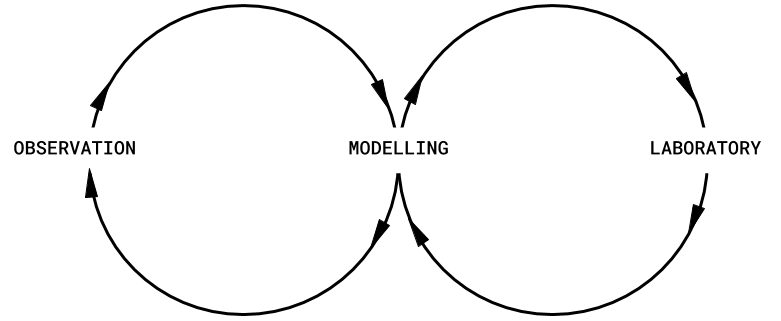
\includegraphics[width=0.6\textwidth]{devcycle.png}
    \caption{\textbf{The scientific development cycle.}This shows the iterative nature between modelling, observation and laboratory experimentation}
    \label{fig:devcycle}
\end{figure}






ESM

 A series of box models.


 \subsection{The Dynamically Simple Model of Atmospheric Chemical Complexity}








 % Early simulations, such
 %
 % as those run on ENIAC2, were capable of success-
 % ful 24 hour weather prediction. Unfortunately, al-
 % though a great feat, the delay in simulation time re-
 % sulted in a computation that only just kept up with
 %
 % real-life events [Lynch, 2008]. in 1995 a general circu-
 % lation model of the atmosphere was created by Phillips
 %
 % [Phillips, 1956]. It was soon discovered that this was
 % insu
 % cient to represent the Earth, and a general Global
 % Climate Model (GCM) was formed from the union
 % of atmospheric, oceanic, cryospheric and land-surface
 %
 % models [NIPCC, 2010]. The outcome of this was a pro-
 % gram capable of simulating accurate short-term weather
 %
 % predictions, which can allow an insight into the con-
 % tributing factors of climate change.
 %
 %
 % \subsubsection{Common Problems with Earth prediction}
 % There are several problems that an earth simulation model can face, most of which can be attributed to computational efficiency. An example of this is seen with the
 %
 % MET - DAY TO SIMULATE
 %
 % Other problems with meteorlogy that are encountered rest on resolution. Too fine a scale and the model can take forever to run. simplfy, lose local effect and islands.
 %
 % Finally the tuning of models can result in overfitting due to a limited understanding or dataset. Here a model may be tweked to ..
 %
 % Numerical stiff chemical complexity.
 %
 %
